\documentclass{standalone}
\usepackage{tikz}

\usetikzlibrary{calc}


\begin{document}

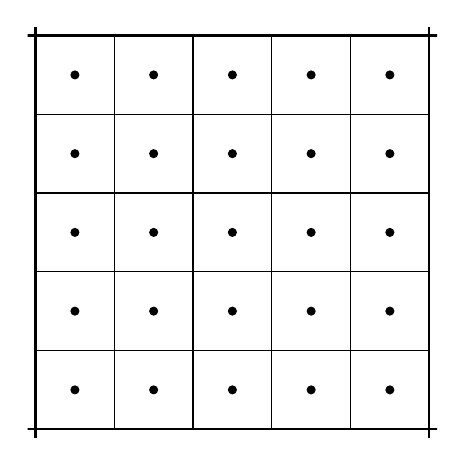
\begin{tikzpicture}
  \path[clip] (-0.1,-0.1) rectangle (5.1, 5.1);
  \draw[thick] (-1,0) -- (6,0);
  \draw[thick] (-1,5) -- (6,5);
  \draw[thick] (0,-1) -- (0,6);
  \draw[thick] (5,-1) -- (5,6);

  \foreach \i in {1,...,5} {
    \draw[thin] (\i,0) -- (\i,5);
    \draw[thin] (0,\i) -- (5,\i);
  }

  \foreach \i in {1,...,5} {
    \foreach \j in {1,...,5} {
      \draw[fill=black] ($ (\i, \j) - (0.5, 0.5) $) circle [radius=0.05cm];
    }
  }
\end{tikzpicture}

\end{document}